\section{Frequenzanalyse}
\subsection{Fourier-Transformation}
\script{121} Um vom Zeitbereich in Frequenzbereich zu Transformieren mitt Funktion $f(t)$ mit der Fourier-Transformation integriert werden:
\[
	F(j\omega) = \int_{-\infty}^{\infty}f(t)e^{-j\omega t}dt
\]

Die Rücktransformation mit der inverse Fourier-Transformation:
\[
f(t) = \frac{1}{2\pi}\int_{-\infty}^{\infty}F(j\omega)e^{j\omega t}d\omega
\]

Die Konvergenzgeschwindigkeit kann im \script{123} nachgelesen werden.

\subsubsection{Eigenschaften}
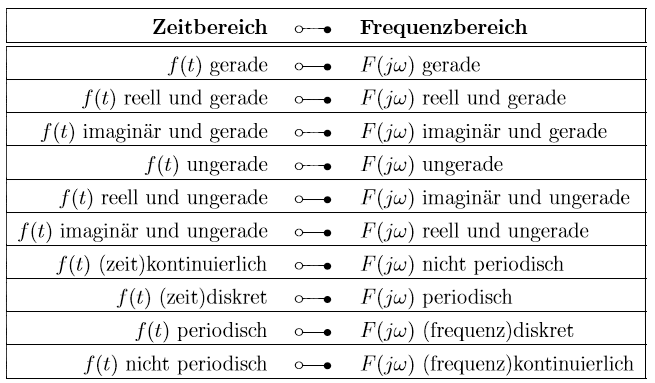
\includegraphics[width=\columnwidth]{Images/fourier_eigenschaten}
Weitere Eigenschaften sind im Skript auf Seite \script{124} zufinden.

\subsection{Laplace-Transformation}
\script{135} Die einseitige Laplace-Transformation transformiert die Zeitdomain in die s-Domain:
\[
F(s) = \int_{0}^{\infty}f(t)e^{-st}dt
\]

\subsubsection{Rücktransformation}
\script{140} Rücktransformation mit \textbf{gebrochen-rationaler Funktionen} ist via PBZ und dem Residuensatz oder mit Tabellen \script{159} zu berechnen:
\begin{align*}
	F(s) = \sum_{i=1}^{k}\sum_{j=1}^{n_k}\frac{A_{ij}}{(s-p_i)^j} \\
	f(t) = \left(\sum_{i=1}^{k}e^{p_it}\sum_{j=1}^{n_k}\frac{A_{ij}t^{j-1}}{(j-1)!}\right)u(t)
\end{align*}

Dabei können die Koeffizienten $A_{ij}$ berechnet werden mit dem Residuensatz:
\[
A_{ij} = \frac{1}{(n_i - j)!}\frac{\partial^{n_i-j}}{\partial s^{n_i -j}}[(s-{p_i})^{n_i}F(s)]|_{s_{p_i}}
\]

\subsubsection{Eigenschaften}
\script{136}
